\subsection{Архитектура решения}

Общая архитектура решения изображена на ~\ref{architecture}. Серым цветом отмечены модули, которые были созданы либо изменены в ходе данной работы.

\begin{figure}[h]
\centering
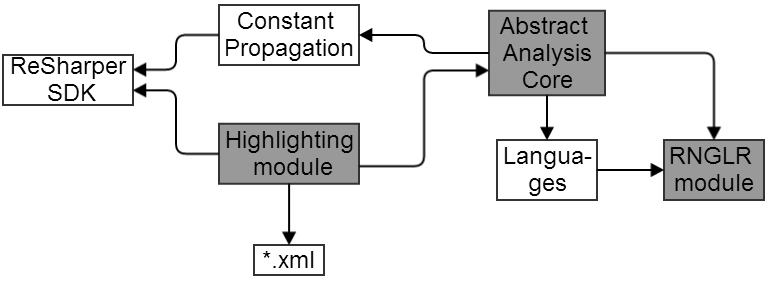
\includegraphics[width=100mm]{Pictures/architecture.png}
\caption{Архитектура решения.}
\label{architecture}
\end{figure}

Рассмотрим эти модули поподробнее. 

Модуль RNGLR содержит в себе функции для работы с графом разбора. В частности он включает реализацию описанных в предыдущей главе алгоритмов извлечения деревьев из SPPF. 

Модуль Languages содержит в себе информацию, специфичную для каждого языка. Например, у каждого языка свой алфавит, свой синтаксический анализатор, своя функция вычисления семантики. Именно такую информацию Languages и хранит. 

Работа модуля AbstractAnalysisCore проходит в два этапа. 

\begin{figure}[h]
\centering
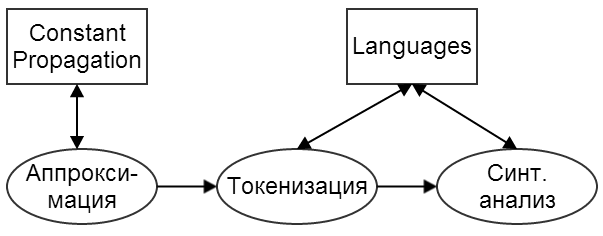
\includegraphics[width=90mm]{Pictures/Core.png}
\caption{Анализ файла модулем AbstractAnalysisCore.}
\label{core}
\end{figure}

На первом этапе происходит анализ файла (рисунок ~\ref{core}). Сперва проходит аппроксимация множества значений строковых выражений, для чего используется другой модуль - ConstantPropagation, целью которого является протягивание констант. Результатом аппроксимации является граф, на рёбрах которого находятся фрагменты строк исходного файла. Также с графом ассоциируется язык, которому соответствуют строки. Далее происходит токенизация полученного графа, в результате которой получается граф, на рёбрах которого находятся токены, а не строки. После токенизации происходит синтаксический анализ. Результат синтаксического анализа - граф разбора - сохраняется. 

\begin{figure}[h]
\centering
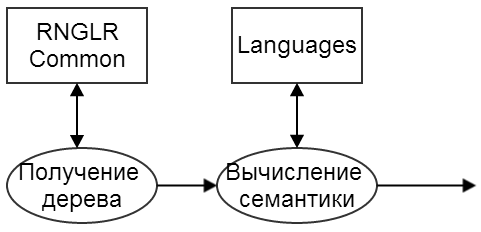
\includegraphics[width=90mm]{Pictures/Core_GetTree.png}
\caption{Получение дерева в AbstractAnalysisCore.}
\label{core_tree}
\end{figure}

На втором этапе работы модуля AbstractAnalysisCore происходит генерация деревьев. Этот этап проиллюстрирован на рисунке ~\ref{core_tree}. Для получения дерева используется модуль RNGLRCommon, который был описан ранее. После того, как дерево получено, происходит вычисление его семантики, и возвращается полученный результат. 

Наконец, модуль Highlighting отвечает за подсветку и интеграцию с ReSharper SDK. Он состоит из трёх подмодулей. Один из них отвечает за статическую подсветку, второй - за динамическую подсветку, а третий (Helper) служит для взаимодействия между ними. 

\begin{figure}[h]
\centering
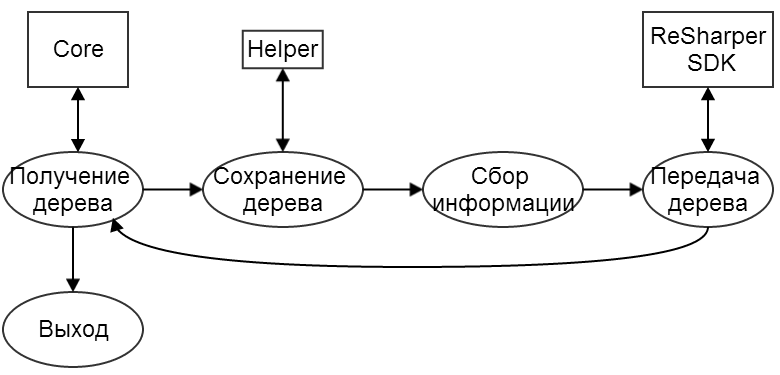
\includegraphics[width=100mm]{Pictures/staticHighlighting.png}
\caption{Схема работы модуля статической подсветки.}
\label{staticHighlighting}
\end{figure}

Схема работы подмодуля, занимающегося статической подсветкой, изображена на рисунке ~\ref{staticHighlighting}. Этот подмодуль начинает работу при каждом изменении файла с исходным кодом. Такое поведение достигается за счёт установления соответствующего атрибута в одном из классов этого подмодуля. Контекст при этом не учитывается. Модуль создаёт инстанцирует класс AbstractAnalysisCore, который проводит синтаксический анализ кода на встроенном языке. После этого возвращается дерево разбора, полученное согласно алгоритму, описанному в разделе 3.2.1. Полученное дерево сохраняется в Helper’е. Далее происходит обход этого дерева, в ходе которого происходит сбор информации о том, какой токен на какой позиции в файле находится. Также каждому токену назначается цвет, в который этот цвет красить (здесь всплывает xml файл, который описан в предыдущем разделе). После этого полученная информация передаётся ReSharper SDK, который осуществляет непосредственную подсветку. И начинается запрос нового дерева. Процесс продолжается до тех пор, пока полученное дерево не является пустым.

\begin{figure}[h]
\centering
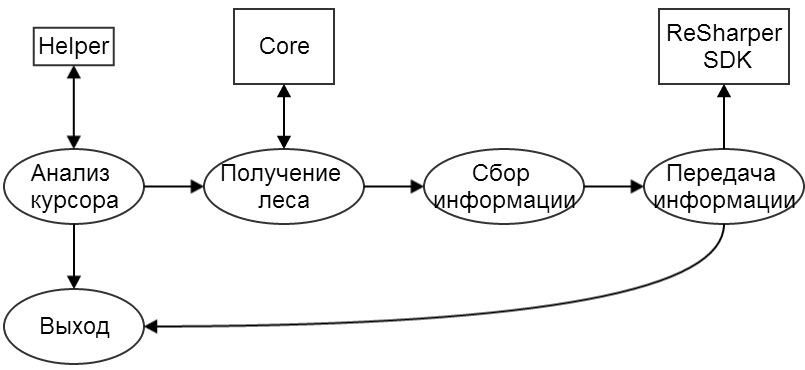
\includegraphics[width=100mm]{Pictures/dynamicHighlighting.png}
\caption{Схема работы модуля динамической подсветки.}
\label{dynamicHighlighting}
\end{figure}

Схема работы подмодуля, занимающегося динамической подсветкой, выглядит несколько иначе (рисунок \ref{dynamicHighlighting}). В отличие от предыдущего модуля он реагирует на каждое изменение положения каретки курсора в файле с исходным кодом. При запуске этого подмодуля сперва происходит анализ положения курсора. Если каретка стоит внутри строкового выражения и перед (после) открывающего (закрывающего) парного символа, то определяется текущий встроенный язык. Это определение происходит за счёт поиска по деревьям разбора, полученным при статической подсветке. Сначала определяется дерево, которое содержит нужный диапазон, а потом по этому дереву определяется, какой именно это встроенный язык. На основе полученной информации у объекта класса AbstractAnalysisCore вызывается функция, которая возвращает все деревья, которые содержат нужный токен. Алгоритм, который используется при этом, описан в разделе 3.2.2. Далее по этим деревьям, так же, как и в работе подмодуля статической подсветки, происходит сбор информации и её передача ReSharper SDK, который подсвечивает парные токены. 

